Este documento tem como objetivo apresentar as atividades realizadas pelo bolsista André Luís Mendes Fakhoury no período de outubro de 2020 a março de 2021, referente ao projeto de Iniciação Científica, processo FAPESP nº 2020/07224-5. O trabalho, intitulado ``Reconstrução de curvas por meio de características robustas extraídas de imagens'', é parte de umas das linhas de pesquisa do projeto temático FAPESP de nº 2019/07316-0, que visa a reconstrução de faces humanas a partir de informações reduzidas do domínio.


\section{O projeto e cronograma original}

Um dos desafios encontrados em visão computacional é o mapeamento de características robustas entre espaços bidimensionais e tridimensionais. Este processo pode ser simplificado com a redução de informações a serem analisadas: como representar curvas a partir de algum conjunto reduzido de pontos.

Este projeto visa, principalmente, a extração de características robustas de curvas, e posterior reconstrução delas a partir destas informações reduzidas com um erro mínimo. Os pontos que representam estas características robustas são denominados pontos importantes.

Para este processo, contornos de imagens podem ser extraídos e analisados como curvas discretas e, portanto, reduzidos a finitos pontos importantes. A partir desta premissa, os seguintes objetivos específicos podem ser definidos:

\begin{itemize}[noitemsep]
	\item Extrair características robustas em $\mathbb{R}^2$ para reconstrução de curvas com alta precisão a partir de imagens. 
	\item Pré-processar as imagens com eliminação de ruídos, binarização e consequente segmentação;
	\item Extrair atributos de formas das imagens (contorno e cálculo da curvatura);
	\item Determinar as características robustas por análise da curvatura;
	\item Reconstruir as formas a partir das características robustas, por meio de curvas poligonais e operadores Laplacianos como sugerido por \citeonline{Sorkine2006} e 
	\item Aferir a qualidade da reconstrução a partir da curva original.
\end{itemize}

As principais etapas de desenvolvimento deste projeto são ilustradas no diagrama de blocos da figura \ref{fig:diagrama}. O projeto, como inicialmente proposto, apresentou o cronograma representado na tabela \ref{tab:cronograma}.

\begin{figure}[htb]
	\centering
	\caption{Diagrama de bloco das etapas de desenvolvimento}
	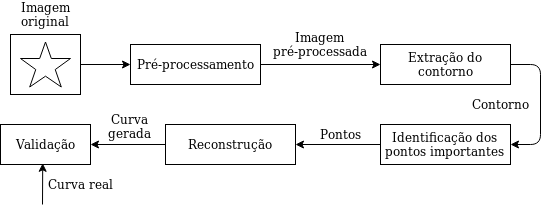
\includegraphics[width=.7\linewidth]{./img/diagrama.png}
	\legend{Fonte: Elaborada pelo autor.}
	\label{fig:diagrama}
\end{figure}



\begin{table}[htb]
	\footnotesize
	\centering
	\vspace{0.5em}
	\setlength{\tabcolsep}{0.05in}
	\begin{tabular}{|c|c|c|c|c|c|c|}
		\hline
		Atividades
		& \multicolumn{6}{c|}{Meses de trabalho} \\
		\cline{2-7}
		& 1\textordmasculine\ e 2\textordmasculine & 3\textordmasculine\  e 4\textordmasculine & 5\textordmasculine\  e 6\textordmasculine & 7\textordmasculine\  e 8\textordmasculine & 9\textordmasculine\  e 10\textordmasculine & 11\textordmasculine\  e 12\textordmasculine \\ \hline
		Estudo das técnicas de reconstrução de curvas  & $\bullet$ & $\bullet$ & & & &\\ \hline
		Pré-processamento e Extração de contornos & & $\bullet$ & $\bullet$ & & & \\ \hline
		Extração dos pontos importantes & & $\bullet$ & $\bullet$ & & & \\ \hline
		Redação do relatório parcial & & & $\bullet$ & & & \\ \hline
		Implementação da reconstrução de curvas & & & & & & \\
		(Sorkine)& & & $\bullet$ & $\bullet$ & $\bullet$ & \\ \hline
		Avaliação e testes & & & & $\bullet$ & $\bullet$ & \\ \hline
		Desenvolvimento do relatório final & & & & & $\bullet$ & $\bullet$ \\ \hline
	\end{tabular}
	\caption{Cronograma de atividades para 12 meses de trabalho.}
	\label{tab:cronograma}
\end{table}

\section{Reordenação do cronograma}\label{sec::reordenacao}

Durante o segundo semestre de 2020, o professor Dr. Antônio Castelo Filho, pesquisador principal do projeto temático, lecionou a disciplina ``Modelagem Geométrica'', de código SME0271, para alunos de graduação e com espelho em ``Tópicos em Análise Numérica II (Variedades Computacionais)'', de código SME5850, para a pós-graduação. Nela, foram abordados diversos tópicos referentes a variedades computacionais. Nas reuniões semanais de acompanhamento das atividades do temático por cada membro da equipe,  o prof. Castelo e demais pesquisadores incentivaram ao aluno bolsista e demais colegas a cursar a disciplina, visto ser uma grande oportunidade para adquirir conhecimento sobre a modelagem geométrica e análise numérica das várias linhas de pesquisas relacionadas. No caso particular deste projeto, a atividade diretamente relacionada referiu-se à reconstrução de curvas pelo método descrito em \citeonline{Sorkine2006}, originalmente programada para ser desenvolvida na segunda metade deste projeto. 

Além do aluno bolsista deste projeto, três alunos de mestrado do projeto temático cursaram a disciplina. Uma das formas de avaliação da disciplina era a co-autoria da escrita de um capítulo de um livro, que ainda será publicado.

Como resultado, a atividade 5 (implementação da reconstrução de curvas) foi antecipada e a atividade 3 (extração dos pontos importantes) postergada para os próximos meses, sem prejudicar o desenvolvimento do projeto. Ressalto que cursar a disciplina foi muito compensador, tendo contribuído para um melhor entendimento da teoria de reconstrução de curvas a partir de um conjunto de pontos e, sobretudo, no momento da implementação, a ser apresentada neste relatório.

\section{Organização do relatório}

As próximas seções deste relatório serão estruturadas da seguinte maneira:

\begin{itemize}[noitemsep]
	\item Na seção \ref{ch::realizadas} serão descritos alguns conceitos estudados e as atividades realizadas;
	\item Na seção \ref{ch::proximas} serão vistas as próximas atividades a serem realizadas;
% 	\item Na seção \ref{ch::consideracoes} serão dadas algumas considerações finais.
\end{itemize}